%%%%%%%%%%%%%%%%
%%%%% Plot %%%%%
%%%%%%%%%%%%%%%%

\chapter{Plotting the Solution} \index{plot|(}

 In the following plotting routines stored in {\tt /Lib/Plots} are explained. They are mostly used to plot the solutions.


%%%%%%%%%%%%%%%%%%%%%%
%% Plot of solution %%
%%%%%%%%%%%%%%%%%%%%%%

\section{Ordinary Plot} \label{sect:plot} \index{plot!solution|(}

 Once the coefficient vector {\tt U} of the finite element solution is computed via the \textbackslash-operator in MATLAB, an illustration is possible using the {\tt plot}-routines saved in the folder {\tt /Lib/Plots}. \\

 The required input arguments are listed in table \ref{tab:plot_in}.

\begin{table}[htb]
  \begin{tabular}{p{1cm}p{10cm}}
    \ttindex{U} & {\small $M$-by-$1$ matrix specifying the values of the coeffiecient vetor at the nodes of the finite element solution} \\
    \ttindex{Mesh} & {\small struct that at least contains the fields {\tt Coordinates} and {\tt Elements} (cf. table \ref{tab:MSH_B}, p. \pageref{tab:MSH_B})}
  \end{tabular}
  \caption{Input for {\tt plot}-routines}
  \label{tab:plot_in}
\end{table}

 The {\tt plot}-functions are e.g. called by \\

\noindent {\tt >> H = \ttindex{plot\_LFE}(U,Mesh);} \\

 Figure \ref{fig:plot_sol} shows the finite element solution of the Laplacian obtained using linear finite elements in \ttitindex{main\_LFE} in {\tt /Examples/QFE\_LFE}. It is plotted using {\tt plot\_LFE}. The colorbar was added separately using the built-in {\tt colorbar}-command in MATLAB. \\

\begin{figure}[htb]
  \centering
  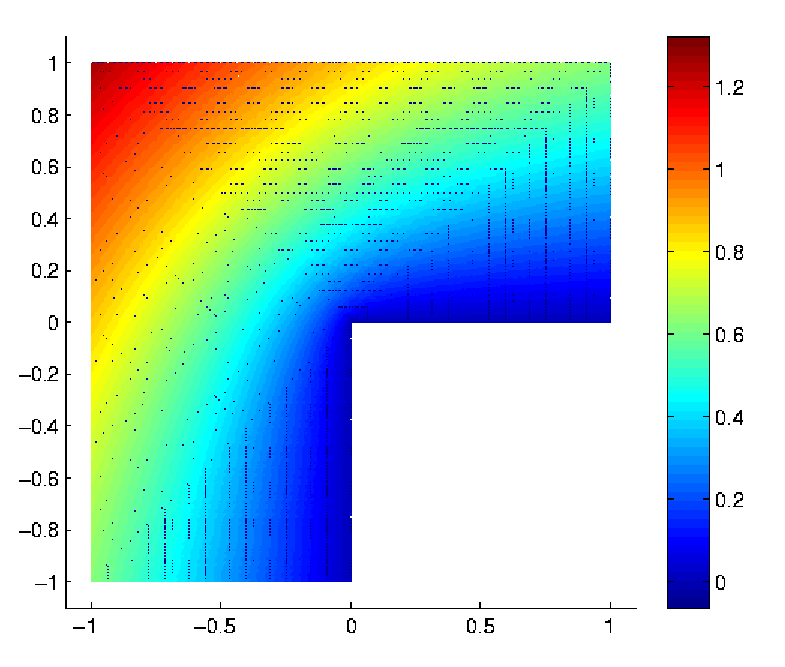
\includegraphics[width=0.5\textwidth]{main_LFE_fig1.eps}
  \caption{Plot of {\tt LFE} solution in {\tt main\_LFE}}
  \label{fig:plot_sol}
\end{figure}

 The function returns a handle to the figure {\tt H}. In case the solution is complex-valued both, the real and imaginary term, are plotted separately. \\

 The following steps are implemented:
\begin{enumerate}
	\item computation of axes limits
	\item plotting of real (and eventually also imaginary) finite element solution using the \MATLAB commands {\tt figure} and {\tt patch}
\end{enumerate}


%% Constant finite elements %%

\subsection{Constant Finite Elements} \index{constant finite elements!plot solution}

 \ttitindex{plot\_P0} generates the plot for the solution on constant finite elements.


%% Linear finite elements %%

\subsection{Linear Finite Elements} \index{linear finite elements!plot solution}

\subsubsection{.. in 1D}

 \ttitindex{plot\_1D} is called by \\

\noindent {\tt >> H = plot\_1D(U,Coordinates);} \\

 where \ttindex{Coordinates} is the $M$-by-$1$ matrix specifying the nodes of the mesh.

\subsubsection{.. in 2D}

 \ttitindex{plot\_LFE} and \ttitindex{plot\_LFEfancy} generate plots of the finite element solution, \ttitindex{plot\_DGLFE} plots the finite element solution for discontinuous linear finite elements. \\

 The solution for vector-valued  linear finite elements is plotted by \ttitindex{plot\_LFE2}.


%% Bilinear finite elements %%

\subsection{Bilinear Finite Elements} \index{bilinear finite elements!plot solution}

 \ttitindex{plot\_BFE} plots the finite element solution computed using bilinear finite elements.


%% Crouzeix-Raviart finite elements %%

\subsection{Crouzeix-Raviart Finite Elements} \index{Crouzeix-Raviart finite elements!plot solution}

 For the plot of the solution computed by Crouzeix-Raviart finite elements, an auxiliary mesh is generated and the solution updated there. The function \ttitindex{plot\_CR} plots the solution, \ttitindex{plot\_DGCR} plots the solution for discontinuous Crouzeix-Raviart elements.


%% Quadratic finite elements %%

\subsection{Quadratic Finite Elements} \index{quadratic finite elements!plot solution}

 In \ttitindex{plot\_QFE} the mesh is refined using \ttindex{refine\_REG} before plotting the finite element solution. See p. \pageref{refine_REG}f for more details on this function.


%% Whitney 1-forms %%

\subsection{Whitney 1-Forms} \index{Whitney 1-forms!plot solution}

 The function \ttitindex{plot\_W1F} generates a plot of the velocity field represented by the W1F solution {\tt U} on the struct {\tt Mesh} and returns a handle to the figure. The functions \ttindex{get\_MeshWidth} and \ttindex{shape\_W1F} are called within the program. The transformation on the reference element is done and there the shape functions and velocity field are computed at its barycenter. Finally, the \MATLAB command {\tt quiver} plots the velocity vectors as arrows. \\

 Note that as usual for the Whitney 1-forms the {\tt Mesh}-fields \ttindex{Edges} and \linebreak 
 \ttindex{Vert2Edge} are needed.


%% hpFEM %%

\subsection{$hp$ Finite Elements} \index{hpFEM@$hp$FEM!plot solution}

\subsubsection{.. in 1D}

 The function \ttitindex{plot\_hp\_1D} generates a plot of the $hp$DG solution {\tt U} on the mesh specified by the $M$-by-$1$ matrix {\tt Coordinates} using the polynomial degrees specified by {\tt p} and the shape functions provided by the function handle {\tt Shap} (cf. \ttindex{shap\_Leg\_1D}, p. \pageref{ssect:shap_Leg}) on each element. It is called by \\

\noindent {\tt >> H = plot\_hpDG\_1D(Coordinates,p,u,Shap);} \\

 The built-in \MATLAB command {\tt plot} is used for the illustration.

\subsubsection{.. in 2D}

 By \ttitindex{plot\_hp} a plot of the piecewise polynomial function of maximum polynomial degree {\tt p} given by {\tt U} on the struct {\tt Mesh} is generated. \\

 In order to split the reference element according to the maximum polynomial degree the function \ttitindex{split\_RefElem} is called. It splits the reference triangle into smaller elements according to the resolution {\tt res} by \\

\noindent {\tt >> [RefCoord,RefElem] = split\_RefElem(res);} \\

 In {\tt plot\_hp} the choosen resolution {\tt res} is {\tt 1/(2*p)}. The \MATLAB command {\tt delaunay} is used to generate the set of triangles such that no data points are contained in any triangle's circumcircle. For details on the output {\tt [RefCoord,RefElem]} of {\tt split\_RefElem} see table \ref{tab:res_out} ($A$ and $B$ depend on the choosen {\tt res}).

 \begin{table}[htb]
  \begin{tabular}{p{2cm}p{9cm}}
    \ttitindex{RefCoord} & {\small $A$-by-$2$ matrix specifying all vertex coordinates} \\
    \ttitindex{RefElem} & {\small $B$-by-$3$ matrix connecting vertices into triangular elements}
  \end{tabular}
  \caption{Output of the function \ttindex{split\_RefElem}}
  \label{tab:res_out}
\end{table}

 On the refined element, the ouput of the shape functions \ttindex{shap\_hp} is computed at the vertices {\tt RefCoord}. Finally, the function values on the elements are computed and then plotted. \\

 The {\tt plot}-function for the $hp$FEM is called by \\

\noindent {\tt >> H = plot\_hp(U,Mesh,Elem2Dof,p);} \\

 The field \ttindex{Elem2Dof} is explained on p. \pageref{elem2dof}.

\index{plot!solution|)}


%%%%%%%%%%%%%%%
%% Plot line %%
%%%%%%%%%%%%%%%

\section{Plot Line} \label{sect:plot_line} \index{plot!line|(}

 The {\tt plotLine}-functions in {\tt /Lib/Plots} generate a plot of the finite element solution {\tt U} on a certain line of the mesh. Again, the solution {\tt U} and the {\tt Mesh} are needed, see table \ref{tab:plot_in}. To specify the line the additional input arguments {\tt x\_start} and {\tt x\_end} are required, see table \ref{tab:plotline_in}.

\begin{table}[htb]
  \centering
  \begin{tabular}{p{1cm}p{10cm}}
    {\tt x\_start} & {\small $1$-by-$2$ matrix specifying the starting point of the section} \\
    {\tt x\_end} & {\small $1$-by-$2$ matrix specifying the end point of the section}
  \end{tabular}
  \caption{Input for {\tt plotLine}-routines}
  \label{tab:plotline_in}
\end{table}

 So far these section plots are implemented for linear and quadratic finite element solutions. The functions are e.g. called by \\

\noindent {\tt >> L = plotLine\_LFE(U,Mesh,x\_start,x\_end);} \\

 Figure \ref{fig:plot_line_sol} shows the output for the Laplacian solved with linear finite elements in \ttindex{main\_LFE} in {\tt /Examples/QFE\_LFE}, cf. figure \ref{fig:plot_sol}. The starting point of the section is $(0,0)$, the end point is $(1,1)$. \\

\begin{figure}[htb]
  \centering
  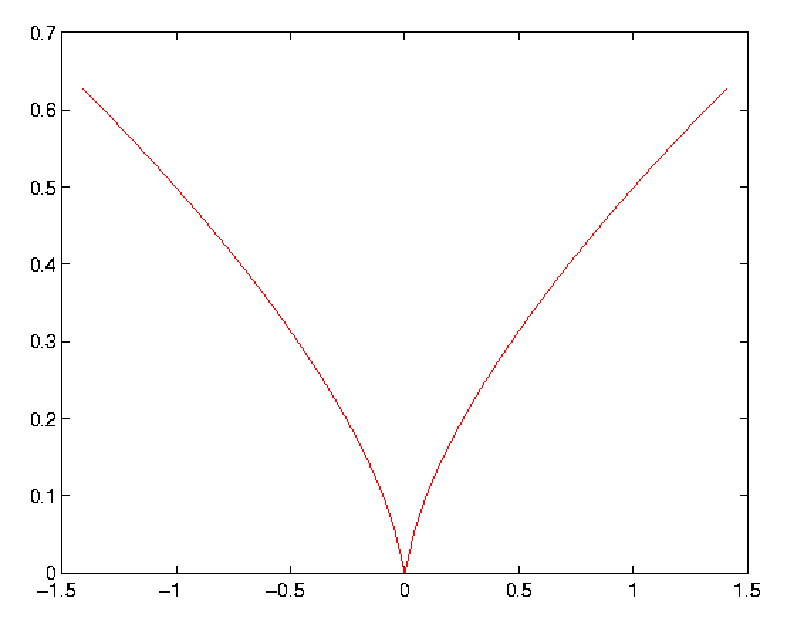
\includegraphics[width=0.5\textwidth]{main_LFE_fig2.eps}
  \caption{Plot section of {\tt LFE} solution in {\tt main\_LFE}}
  \label{fig:plot_line_sol}
\end{figure}

 The element contributions are computed using the specific shape functions, cf. section \ref{sect:shap}. The figures are generated by the \MATLAB command {\tt plot}.


%% linear finite elements %%

\subsection{Linear Finite Elements} \index{linear finite elements!plot section of solution}

 The function \ttitindex{plotLine\_LFE} plots the finite element solution on the desired section using \ttindex{shap\_LFE} to compute the element contributions.


%% quadratic finite elements %%

\subsection{Quadratic Finite Elements} \index{quadratic finite elements!plot section of solution}

 Similarily, \ttitindex{plotLine\_QFE} calls \ttindex{shap\_QFE} to compute the element contributions on the section specified.

\index{plot!line|)}


%%%%%%%%%%%%%%%%%%%
%% Plot contours %%
%%%%%%%%%%%%%%%%%%%

\section{Plot Contours} \label{sect:plot_contour} \index{plot!contours|(}

 The {\tt contour}-functions in the folder {\tt /Lib/Plots} generate a contour-plot of the finite element solution {\tt U} on the {\tt Mesh}, see table \ref{tab:plot_in}. The functions are called by \\

\noindent {\tt >> H = \ttindex{contour\_LFE}(U,Mesh);} \\

 where {\tt H} is a handle to the generated figure. Further variable input arguments are listed in table \ref{tab:plot_add}.

\begin{table}[htb]
  \begin{tabular}{p{2cm}p{9cm}}
    {\tt levels} & {\small vector that specifies at which values contour lines should be drawn} \\
    {\tt 'c'} & {\small specifies the color of the level curves. See \MATLAB help for colorspec for predefined colors.
   The default color is {\tt 'b'} (blue).} \\
    {\tt 'colorbar'} & {\small appends a colorbar to the current axes in the right location}
  \end{tabular}
  \caption{Additional input for {\tt contour}-routines}
  \label{tab:plot_add}
\end{table}

 Hence the differing calls are e.g. \\

\noindent {\tt >> H = contour\_LFE(U,Mesh,levels);} \\
\noindent {\tt >> H = contour\_LFE(U,Mesh,levels,'c');} \\
\noindent {\tt >> H = contour\_LFE(U,Mesh,levels,'colorbar');} \\

 Figure \ref{fig:plot_cont_sol} shows the output of the function \ttitindex{main\_ContourExample} stored in the folder {\tt /Examples/QFE\_LFE}. It's the solution of the Laplacian using linear finite elements, cf. figures \ref{fig:plot_sol} and \ref{fig:plot_line_sol}.

\begin{figure}[htb]
  \centering
  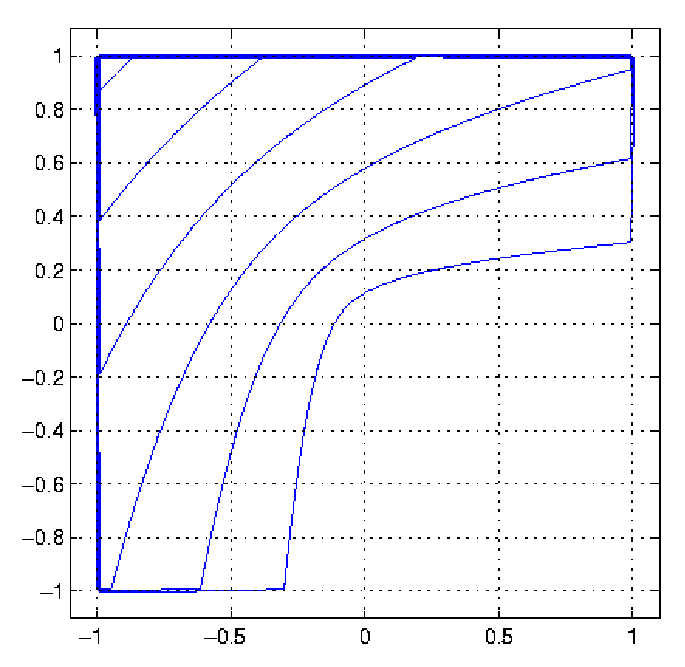
\includegraphics[width=0.5\textwidth]{main_ContourExample.eps}
  \caption{Contour plot of {\tt LFE} solution in {\tt main\_ContourExample}}
  \label{fig:plot_cont_sol}
\end{figure}


%% Linear finite elements %%

\subsection{Linear Finite Elements} \index{linear finite elements!contour plot of solution}

 By \ttindex{get\_MeshWidth} the mesh width for a given triangular mesh is computed. For each element, the coordinates of the vertices are extracted, the element mapping is computed and the element transformed to the reference element using the shape functions in \ttindex{shap\_LFE}. The solution is then plotted using the \MATLAB command {\tt contour}. All this is done by the function \ttitindex{contour\_LFE} which may be called as explained above. \\

 An application of {\tt contour\_LFE} is included in \ttitindex{main\_ContourExample} which is stored in the folder {\tt /Examples/QFE\_LFE}.


%% Crouzeix-Raviart finite elements %%

\subsection{Crouzeix-Raviart Finite Elements} \index{Crouzeix-Raviart finite elements!contour plot of solution}

 As above the solution in \ttitindex{contour\_DGCR} is computed using transformed grid points by \ttindex{shap\_DGCR}. \\

 The function is used to plot the approximate solution for the circular advection problem \ttindex{main\_CA\_2} stored in {\tt /Examples/FVDG}.

\index{plot!contours|)}

%% Plane wave DG %%

%\subsection{Plane wave DG}

%\ttitindex{contour\_PWDG}


\index{plot|)}